\chapter{Object Reconstruction and Event Generation}
\label{chap:event_sim}
\epigraph{Any one who considers arithmetical methods of producing random digits is, of course, in a state of sin. For, as has been pointed out several times, there is no such thing as a random number --- there are only methods to produce random numbers, and a strict arithmetic procedure of course is not such a method.}{\textit{Jon von Neumann}}
\vskip 0.5in
\section{Introduction}
\label{intro}
This chapter is divided into two parts. In the first part, the procedure for the generation of simulated events is described. This is done in several distinct stages with the output of one stage serving as an input for the next. A suite of software packages, developed mostly by the particle and nuclear physics communities, is used to achieve this. This part concludes by detailing the simulated datasets used in the analyses described in this thesis. In the second part of this chapter, the reconstruction of physics objects is described in detail. It starts with a description of the particle-flow algorithm which is a global event reconstruction scheme for the entire event. This is followed by descriptions of track, muon and electron reconstructions. Reconstruction of jets is described next followed by description of composite objects used in the analysis such as collinear mass and transverse mass.
 

\section{Event simulation}
A $pp$ collision at the LHC, like any hadronic collision, is more complex than the hard interaction of two participating partons. The proton being a composite object, the colliding partons from the hard interaction are accompanied by other quarks and gluons that interact and rearrange themselves into color singlets due to color confinement. A $pp$ collision thus consists of: the Hard Scattering which represents the part of the collision where two partons in the initial state interact by exchanging high transverse momentum, and the Underlying Event that represent the interaction of the everything else in the collision except the partons in hard scattering. In addition to the implementing the above, i.e. physics of a $pp$ collision  that produces a bunch of final state particles, the event simulation also has to include interactions of these particles with the CMS detector. Monte Carlo methods, that use generation of random numbers to simulate sampling from a given probability distribution, are used to model the above event simulations~\cite{mc_evtsim}.

\subsection{Monte Carlo method}

Monte Carlo (MC) methods (named after a famous casino in the city state of Monaco) are a broad class of computational algorithms that rely on repeated random sampling to obtain numerical results~\cite{mcwiki}. In particle physics, these methods play a key role in generation of events and are used primarily for : generation of samples from specified probability distributions, and the calculation of integrals. Programs which implement the above method, called MC event generators, use generation of random numbers to make decisions about physics processes. These can range from selection of processes that are generated in the collision, to which decay channel a particle decays in, to making decisions on how the particle interacts with detector material. Usually, each such decision is the result of a draw from a distribution which depends only on the current state the process is in, and not on previous states. The MC generator is provided as input the distributions that represent the physics of the generated particles, their production, their decay modes and their couplings. A MC generator starts by using a pseudo-random number generator that usually outputs a random number between 0 and 1. Although, true random number generation can only be done by physical processes, modern pseudo-random number generators are known to generate numbers with a high degree of randomness. Starting from this distribution, the MC event generator uses one of the various methods such as the inverse-transform method, or the rejection sampling method to convert this uniform distribution into a desired probability distribution, $p(x)$. It is then possible to generate random numbers according to this distribution to simulate physical processes. 


\subsection{CMS simulation pipeline}

The MC simulation of events in CMS consists of the following sequential steps. The first step is simulation of the Hard Scattering. As mentioned earlier, this represents the primary hard interaction in a collision where two partons in the initial state interact by exchanging high transverse momentum resulting in a final state with two or more partons. The parton density function (pdf) which parametrizes the distributions of the partons inside each hadron are used to model the momenta of incoming partons. It represents the probability of finding a parton of a certain flavor at a certain longitudinal momentum fraction, when the hadron, that contains it, is probed at a certain scale. The PDF are extracted from fits to the data, mainly from ep collisions, and various PDF sets are available for each parton flavor. Commonly used pdf sets include ones provided by the  CTEQ, HERA (H1 and ZEUS) and NNPDF collaborations. The LHAPDF library provides a unified C++ interface to all major PDF sets. The matrix element formulation is used to model the hard scattering process to leading order in perturbative QCD, or to higher orders depending on the generator. The next step is simulation of the parton shower. The hadronization and radiation of quarks and gluons in the initial and final states cannot be feasibly encapsulated in the matrix element computation. Parton shower describes these missing parts. The matrix element calculations are combined with the parton shower by one of the different matching schemes which ensure that there is no double counting of terms present in both the matrix element and the parton shower expansion. The matching schemes that are most often used are MLM~\cite{mlm}, CKKW~\cite{ckkw} and FxFx~\cite{Frederix:2012ps}. The simulation of the Underlying Event comes next. Underlying event includes everything in the collision that is not associated with the primary hard scattering process. This consists mostly of soft QCD interactions, and implemented using the MC event generators and interfaced with the matrix element simulation. The hadronization of the quarks and gluons is simulated next and it consists of recombination of individual partons into colorless hadrons. Lastly, the decay of short-lived particles is simulated.

An important part of the event generation chain is the simulation of pileup. The protons circulate inside the LHC not as a continuous beam but in discrete closely packed bunches. This leads to more than one proton-proton collision per bunch crossing, i.e. pileup both in-time and out-of-time (see chapter~\ref{chap:exper_setup}). Event generators add  pile-up events to the hard scattering samples by randomly simulating soft inelastic collisions and overlapping them. The distribution of the number of pileup interactions in data is hard to predict. MC event generators usually produce events for a scenario with a higher number of pileup vertices, and with a flat distribution of number of vertices . This is afterwards reweighted to match the observed distribution of pileup interactions in data.

Several MC generators have been developed. Some of these can produce all components of the above simulation pipeline while some calculate only the matrix element and need to be interfaced with other generators for the simulation of remaining parts. Pythia~\cite{Sjostrand:pythia8} and Herwig~\cite{herwig} can produce the entire chain while Powheg~\cite{Nason:2004rx,Frixione:2007vw, Alioli:2010xd, Alioli:2010xa, Alioli:2008tz, Bagnaschi:2011tu}, aMC@NLO~\cite{Alwall:2014} and Madgraph~\cite{Alwall:2011uj} produce up to matrix element stage. Powheg and aMC@NLO can perform next-to-leading order calculations. 

Finally, the Geant4 (GEometry ANd Tracking)~\cite{GEANT4} package is used to simulate the interaction of physical particles after the collision, produced by pipeline described  above, with a sophisticated and complex simulation of the detector itself. This simulated detector response is used as input for the same physics reconstruction algorithms (described in the next section), that are used to reconstruct the data, thus enabling a direct comparison of the two. If differences are observed in the behavior of these reconstruction algorithms for MC events in comparison to observed data, the MC events are tuned to the behavior observed in data. 


\section{MC samples used for the analyses}
\label{samples_mc}

The {ggH} and VBF Higgs boson samples are generated with POWHEG 2.0 while an extension of POWHEG 2.0~\cite{Luisoni:2013kna} is used for the $\PW\PH$ and $\PZ\PH$ simulated samples. For the \Hmue analysis, only the gluon fusion (ggH) production mode has been considered. Samples are generated for a range of H masses from 200 to 900 GeV.

The $\zjets$ and $\wjets$ processes are simulated using the \aMCATNLO generator at leading order (LO) with the MLM jet matching and merging scheme. The same generator is also used for diboson production which is simulated at  next-to-LO (NLO) with the FxFx jet matching and merging scheme. POWHEG 2.0 and 1.0 are used for top quark-antiquark ($\ttb$) and single top quark production, respectively. The POWHEG and MADGRAPH generators are interfaced with PYTHIA 8 for parton showering, fragmentation, and decays. 

As mentioned earlier in this chapter, additional pileup interactions are also a part of the MC generation pipeline. All simulated samples are reweighted to the pileup distribution observed in data. An event weight is applied based on the number of simulated pileup events and the instantaneous luminosity per bunch-crossing, averaged over the run period. Several other scale factors  are used to reweight the events in order to get the MC simulation to match the data closely. These include scale factors based on trigger, lepton identification, lepton isolation and b-jet tagging efficiencies.

\section{Physics object reconstruction}
\label{p_ob_recon}
This section begins with the description of the particle-flow algorithm followed by reconstruction of tracks and vertices, electrons, muons, jets and other physics objects.  
\subsection{Particle flow}
\label{p_flow}
The overarching algorithm used by CMS to produce a unified global (synchronized for all sub-detectors) description of an event is the particle-flow (PF) algorithm~\cite{Sirunyan:2017ulk}. The idea behind the PF algorithm is that if the basic building blocks or elements from the various sub-detectors can be correlated in a well-defined way, then the description of the event and that of each particle in it can be refined by using the global information from the entire detector. The ALEPH experiment at the CERN LEP collider was the first experiment to use such a holistic approach towards event reconstruction. The CMS experiment, owing to its very  granular layers of sub-detector, is the first hadron collider experiment to successfully use particle-flow. The first step of the PF algorithm is the linking of the several building-blocks or PF elements that a single particle can give rise to, across different sub-detector layers. The link algorithm tests pairs of neighbors in the $\eta-\phi$ plane and combines (links) them to form PF blocks. Reconstruction and identification algorithms are run according to a predefined sequence in each of these PF blocks. First, muon candidates are reconstructed and identified. If a muon candidate successfully passes PF quality criterion, the PF elements associated with it are removed from the block. Electron reconstruction proceeds next with electron candidates successfully becoming PF electrons  if their tracks in the tracker, when extrapolated,  have a corresponding energy deposit in the ECAL. The reconstruction procedure of muons, electrons and tracks are discussed in detail in the sections ~\ref{mu_recon},~\ref{track_recon},~\ref{e_recon}. The PF block now consists of photons and hadrons. To reduce fake track identification, tracks with momentum uncertainty larger than the resolution of the calorimeters are removed at this stage. The remaining tracks are then associated with charged hadrons. The remaining calorimeter energy deposits are then associated with photons (ECAL) and hadrons (HCAL). In this manner, PF finally produces a list of all electrons, photons, muons, charged hadrons and neutral hadrons in the event with optimally determined direction, charge and energy.          



\subsection{Track and primary vertex reconstruction}
\label{track_recon}

Tracks of charged particles, that traverse the CMS tracker (described in section~\ref{tracker}), are reconstructed~\cite{track_reconstruction} using hits from the pixel and strip detectors in the tracker. Hits are reconstructed by clustering signals above specified thresholds in the pixel and strip channels, and then estimating the cluster positions and uncertainties in a local orthogonal system plane of each sensor. During track reconstruction, a translation is made between the local coordinate system of these hits to the global coordinate system of the tracks. The software used to reconstruct tracks by CMS is called the Combinatorial Track Finder (CTF) and is adaptation of the Kalman filter~\cite{kalman_filter}. Tracks are reconstructed using a iterative procedure with the basic idea being, tracks that are easiest to find (e.g., high $\pt$ tracks, and tracks produced near the interaction region) are searched in the initial iterations, with subsequent iterations looking for more difficult sets of tracks (e.g., low $\pt$ tracks , or tracks produced far from the interaction region). Hits unambiguously assigned to the track in the previous iterations are removed for the subsequent ones, thus reducing the combinatorial complexity. Each iteration can be divided into four sequential steps.

The first step is seed generation which provides initial track candidates that define the starting trajectory parameters and associated uncertainties of potential tracks. Charged particles follow helical paths in the quasi-uniform magnetic field of the tracker, requiring a total of five parameters to determine the trajectory. These five parameters are extracted using two or three hits in the inner region of the tracker. The seeds are constructed in the inner part (and then tracks constructed outwards, and not in the opposite manner) because the high granularity of pixel detectors (in contrast to outer strip layers)  ensure that low fraction of channels are hit. Also, particles like pions and electrons interact inelastically with tracker material or lose energy due to bremsstrahlung radiation as they traverse through the tracker to its outer regions, making the idea of constructing seeds in the inner region a better choice.

The second step in track generation is track finding which is closely based on the Kalman filter. It extrapolates the seed trajectories along the expected path of a charged particle, beginning with an estimate of the track parameters provided by the trajectory seeds generated in the last step. It then uses the location and uncertainty of detected hits, and estimations of effects such as Coulomb scattering, at successive detector layers, to build track candidates, updating the parameters at each layer. First, using the parameters of the track candidate, evaluated at the current layer, an analytical extrapolation is done that determines which adjacent layers of the detector the trajectory can intersect. This takes into account the current uncertainty in that trajectory just like a Kalman filter. Secondly, a search is performed for silicon modules in these layers that are compatible with the extrapolated trajectory. All compatible modules in each layer are then grouped into mutually exclusive groups, such that no two modules in each group overlap. The collection of all hits from from one such module group forms a group of hits. Finally, new track candidates are formed by adding exactly one of the compatible hits from each group, to each original track candidate. The modules in a given group are mutually exclusive and a contribution of more than one hit from each group is not expected. The trajectory parameters of the new candidates are then updated by combining the information from the added hits with the extrapolated trajectory of the original track candidates. Figure~\ref{fig:trackrecon} illustrates the reconstruction efficiency of tracks in case of isolated muons.

The third step in track generation track fitting. In this step the collection of hits from the last step are refitted using a Kalman filter and smoother, to provide a best possible estimate of parameters for each track trajectory. The procedure described above, in conditions as challenging as the LHC, can yields several fake tracks that are not associated with any charged particle passing through the tracker. The fourth and final step applies several quality requirements to the set of reconstructed tracks and substantially reduces the fake contribution. The requirements are based on criteria such as the minimum number of layers the track has hits in, how compatible its origin is with a primary vertex, how good a fit it yields etc.

\begin{figure*}
\begin{center}
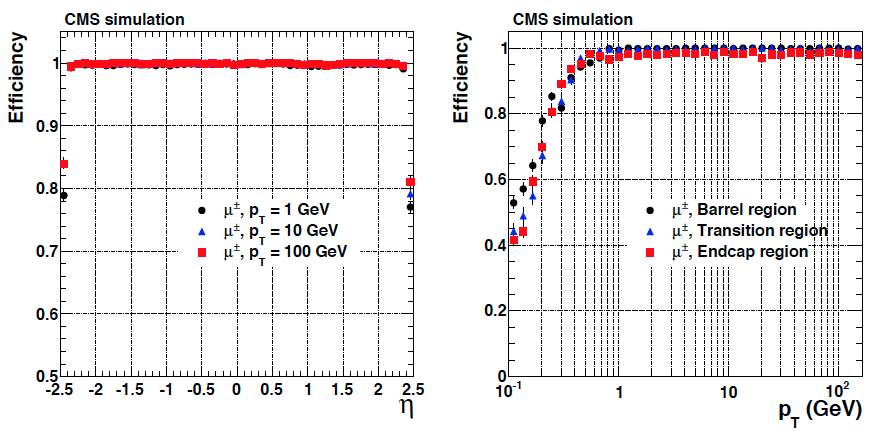
\includegraphics[width=0.9\textwidth,keepaspectratio]{plots_and_figures/chapter4/trackrecon.png}
\caption{Track reconstruction efficencies for single isolated muons as a function of $\eta$ and \pt~\cite{track_reconstruction}.}
\label{fig:trackrecon}
\end{center}
\end{figure*}


Proton-proton interaction vertices are reconstructed by selecting tracks that are produced promptly in the primary interaction region. The selected tracks are then clustered on the basis of their z-coordinates at their point of closest approach to the centre of the beam spot, which represents a 3-D profile of the region where the LHC beams collide inside the CMS detector. The exact positions of the vertices are then obtained from these clustered candidates, by using a fitting procedure, called the adaptive vertex fitter~\cite{vertex_fitting}. The vertex which has the largest sum of squared transverse momenta of tracks originating from it is considered the primary interaction vertex. 


\subsection{Muon reconstruction}
\label{mu_recon}
Hits in the muon system (described in section~\ref{muon_system}) and tracks (muons being charged particles leave tracks in the tracker) from the tracker are used to reconstruct muons~\cite{muon_recon2018}. When muons traverse a muon subdetector (such as RPC, CSC or DT) in the muon system, they ionize the gas in the chambers. The electrical signals produced on the wires and strips as a consequence of the ionization are read out by electronics systems that associate these ``hits'' with well-defined locations in the detector. Various algorithms depending on the subdetector technology are used to reconstruct these hits. Reconstruction of muon tracks using these hits first proceeds independently of track reconstruction in the tracker. These tracks, called \textit{standalone-muon tracks}, are built using these reconstructed hits from the muon system using a Kalman filter. Muon tracks are also built inside-out by propagating tracker tracks (described in previous section) with transverse momentum above 0.5 GeV to the muon system and matching them to (straight-line) segments of hits in DT or CSC. If a match is found, the tracker track qualifies as a \textit{tracker muon track}. Muon tracks are also  built outside-in  by matching standalone-muon tracks with tracker tracks, and combining information from both using a Kalman filter fit. These are called \textit{global muon tracks}. The global muon reconstruction is especially efficient for muons leaving hits in several muon stations. The \textit{tracker muon} reconstruction is more efficient for low $\pt$ muon candidates but it can cause fake muon tracks due to hadronic particles which \textit{punch-through} to the innermost muon stations. The \textit{global muon} reconstruction has  high efficiency for muons penetrating through more than one muon station, and reduces the muon misidentification rate compared to tracker muons. Combining both \textit{tracker muon tracks} and \textit{global muon tracks}, the efficiency for reconstructing a muon is as high as 99\%. The particle-flow algorithm applies a set of requirements, based on various quality parameters from muon reconstruction as well as information from other sub-detectors, to reconstructed candidates. The PF muon candidates used in the analyses described in this thesis were required to satisfy the following set of criterion to be identified as a muon:

\begin{itemize}
\item Must be a global muon or a tracker muon.
\item Must have at least one hit in the pixel subdetector of the tracker
\item $\chi^2$ of the compatibility between the position of the standalone and trackers tracks $<12$
\item Transverse impact parameter of the associated tracker track with respect to the primary vertex $d_{xy}< 2 mm$
\item Longitudinal distance of the (origin of )associated tracker track with respect to the primary vertex $d_z <5 mm$
\item constraints on muon segment matching compatibility between tracker and muon system dependent on if it is a global muon
\end{itemize}
The efficiency of the above selection for muon identification is illustrated using a plot from a study performed by the CMS Muon Physics Object group in Fig.~\ref{fig:muoneff}. As can be seen from the plots, there is a difference in the efficiencies in data and MC simulation. This is corrected using a set a of scale-factors applied as a function $\eta$ and $\pt$ to adjust the efficiency in simulation to get it to match the efficiency in data.  

\begin{figure*}[!htpb]\centering
 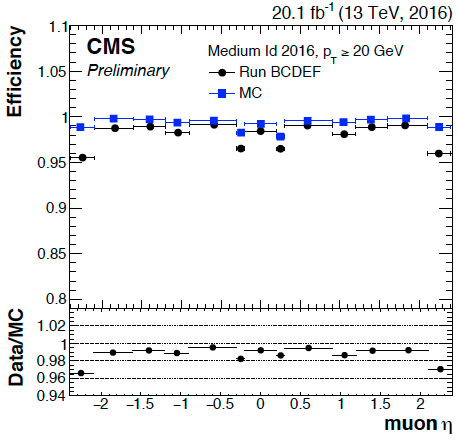
\includegraphics[width=0.47\textwidth]{plots_and_figures/chapter4/muoneffveta.png}
 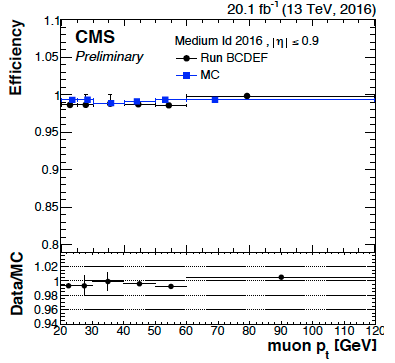
\includegraphics[width=0.49\textwidth]{plots_and_figures/chapter4/muoneffvpt1.png} \\
 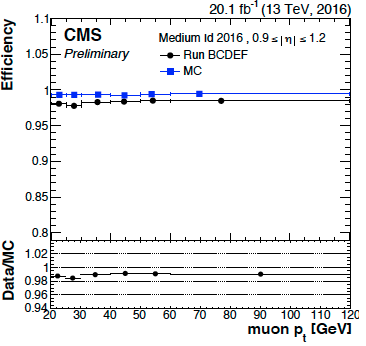
\includegraphics[width=0.49\textwidth]{plots_and_figures/chapter4/muoneffvpt2.png}
 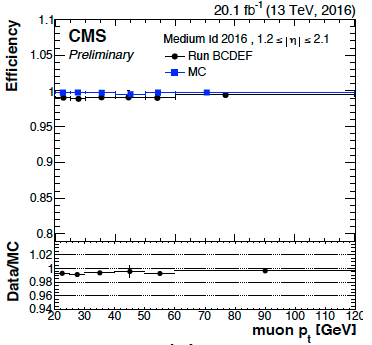
\includegraphics[width=0.49\textwidth]{plots_and_figures/chapter4/muoneffvpt3.png} 
\caption{Efficiency of muon identification as a function of $\eta$ and $\pt$, for data (black) and simulation (blue)~\cite{muon_pog}}
 \label{fig:muoneff}
\end{figure*}  
  
The momentum of muons is measured by CMS using one among different possible ways involving the tracker and muon system~\cite{muon_recon2012} and then using the PF algorithm to refine this measurement exploiting information from the full event.



\subsection{Electron reconstruction}
\label{e_recon}
Besides muons, electron form the other primary part of the final state of the decay we are searching for in this thesis. Electrons, in the CMS, are reconstructed using clusters of energy formed in the ECAL (described in section ~\ref{Ecal}) and associating them with tracks from the tracker~\cite{e_recon}. The reconstruction of electrons is made complicated by the fact that they can radiate a significant amount of energy before reaching the ECAL. This happens due to the radiation of bremsstrahlung photons caused by the interaction of electrons with atoms as they pass through the tracker. This loss can range from 33\% to as high as 86\% depending on $\eta$ (as a consequence of the fact that the amount of detector material the electron has to cross is $\eta$ dependent). In order to measure the an electron's energy,  clustering algorithms thus need to take into account the energy from these bremsstrahlung photon showers, together with the deposit made in the ECAL by the electron. The energy from these radiated photons spreads primarily in the $\phi$ direction, owing to bend in electron trajectory in the magnetic field of CMS. The spread in the $\eta$ direction is relatively small. These facts are used by the clustering algorithms.

The algorithm used to cluster the electron energy deposit in the ECAL barrel is called the \textit{hybrid} algorithm. It exploits the above property of the electron shower shape, and uses the geometry of the ECAL to form clusters that are narrow in $\eta$ direction but wide in $\phi$ direction. Starting with a (seed) crystal containing the largest amount of energy deposited in a considered region above a certain threshold (1 GeV), it adds 5x1 arrays of crystals in $\eta\times\phi$ around the seed crystals in both directions of $\phi$ if the energy contained in the arrays is above another predefined threshold (0.1 GeV). Contiguous arrays are merged into clusters, and finally a electron supercluster is formed from all such strip clusters which have at least one seed strip with energy above another predefined threshold (0.35 GeV). The position of the supercluster is computed as the energy-weighted mean of the cluster positions, whereas its energy is simply taken as the sum of the energy of all its constituent clusters. In the ECAL endcap a different clustering algorithm is used owing to different geometrical arrangement of the crystals. This algorithm called the 5x5 algorithm starts similarly with a seed crystal with maximum energy in a local region, and satisfying the minimum energy requirement of 0.18 GeV. Clusters of 5x5 crystals are progressively grouped around the seed crystal, making a supercluster, if the total cluster energy exceeds 1 GeV and they are within $\pm 0.7$  and $\pm 0.3$ respectively in $\eta$ and $\phi$ around the seed crystal. The position and energy of the supercluster is calculated in the same manner as the barrel. The energy from the preshower is also added into the supercluster, using it's most energetic cluster and it's maximum distance in $\phi$ to other clusters, and extrapolating it to the preshower plane to define the spread in the preshower. The thresholds used in the above algorithms were optimized using simulation and adjusted during data taking periods.

The standard track reconstruction (section~\ref{track_recon}) is not efficient for electrons. This is because the standard approach is compromised by the large radiative losses in the tracker leading to a poor estimation of track parameters~\cite{track_reconstruction}. Therefore, a dedicated tracking procedure is used for electron candidates that uses information not only from the tracker but also the ECAL. Just like the standard track reconstruction procedure, the first step in electron track reconstruction is seeding. This is done in two ways and the results are then combined. In the first method, superclusters from ECAL are used. As mentioned earlier, owing to strong magnetic field, the bremsstrahlung photons emitted by the electrons deposit energy in the ECAL at $\eta$ values similar to that of the electron, but at different $\phi$ leading to a spread. The ECAL supercluster algorithms described above recover this energy. The position and  energy of these reconstructed superclusters along with the assumption that the electrons originated close to the center of the beam spot can be used to constrain the trajectory of the electron through the tracker. Hits in the first layers of the trackers compatible with these trajectories are deemed electron seeds. In the second method of seeding, the ``opposite'' is done. Tracks constructed by the regular tracking algorithm are extrapolated to the ECAL and matched with a supercluster. The seeds corresponding to such matching tracks are retained as electron seeds. The seed collections from these two methods are merged leading to a increase in overall efficiency of the seeding procedure. These seeds are then used to initiate electron track finding and fitting phases. This track finding procedure is similar to that used in standard tracking except for small adjustments. The $\chi^2$ fit thresholds used by the Kalman filter to decide whether a hit is compatible with a trajectory (see section~\ref{track_recon}) is weakened to accommodate tracks that deviate from their expected trajectory because of bremsstrahlung. Similar adjustments are made to the penalties assigned to track candidates for passing through a tracker layer without being assigned a hit. The final track fit uses a modified version of the Kalman filter, called the Gaussian Sum Filter (GSF), to account for the fact that the energy loss of an electron traversing the tracker material is non-Gaussian. This  makes it unsuitable to use a conventional Kalman filter algorithm which assumes gaussian distribution. The GSF technique deals with this by approximating this non-Gaussian energy-loss distribution as the sum of several Gaussian functions, and is found to perform much better than the regular fitting procedure.

Finally, electron candidates are constructed by associating a electron track (called GSF track) produced by the above procedure with a supercluster in the ECAL. For ECAL-seeded candidates this association is made by a geometrical matching in $\eta-\phi$, while for tracker-seeded candidates a multivariate (MVA) technique that combines information from supercluster and GSF track is used. The electron charge is estimated using a combination of three procedures involving the use of the GSF track curvature, use of ECAL supercluster position and its relative position in $\phi$ to that of the first hit in the GSF track, and also by using KF tracks that have common hits with the GSF tracks. The combination of a best vote of three methods reduces the charge misidentification probability to 1.5\%  compared to 10\% when using just the GSF track curvature method. Like other variables, the momentum of electrons is also estimated using a combination of tracker and ECAL measurements.


Further, several quality requirements are used on reconstructed electron candidates to identify (real/signal) electrons to suppress fake sources such as photon conversions, jets misidentified as electrons etc.
These requirements are based on variables that fall into three broad categories: variables that compare measurements from ECAL and the tracker, variables that come only from ECAL (such as transverse shape of electromagnetic showers, ratio of energy fractions deposited in the HCAL to the ECAL ) and purely tracking based variables (such as information from GSF track, difference between the information from GSF and KF-fitted tracks). These variables can be used in two ways: a cut-based method that uses the variables above directly to apply threshold requirements, or a multivariate (MVA) technique that uses all these variables as an input to a Boosted Decision Trees classifier to obtain a combined discriminator variable on which a threshold is applied. The BDT based method has much better performance as is illustrated in Fig~\ref{fig:elec_eff}. Two separate BDTs are trained depending on whether electron is required to pass a HLT triggering requirement or it is not. The trigger selection used in the analyses described in this thesis uses trigger based on muons. The BDT based identification criterion for non-triggering electrons is thus used in this analysis. The threshold corresponding to the working point used in this analysis has an efficiency of approximately 80\%. The difference in efficiencies  of electron identification based on the above criteria in data and MC simulation is corrected using a set a of scaled factors, applied as a function $\eta$ and $\pt$. This adjusts the efficiency in simulation to get it to match the efficiency in data.  
   

\begin{figure*}[!htpb]\centering
 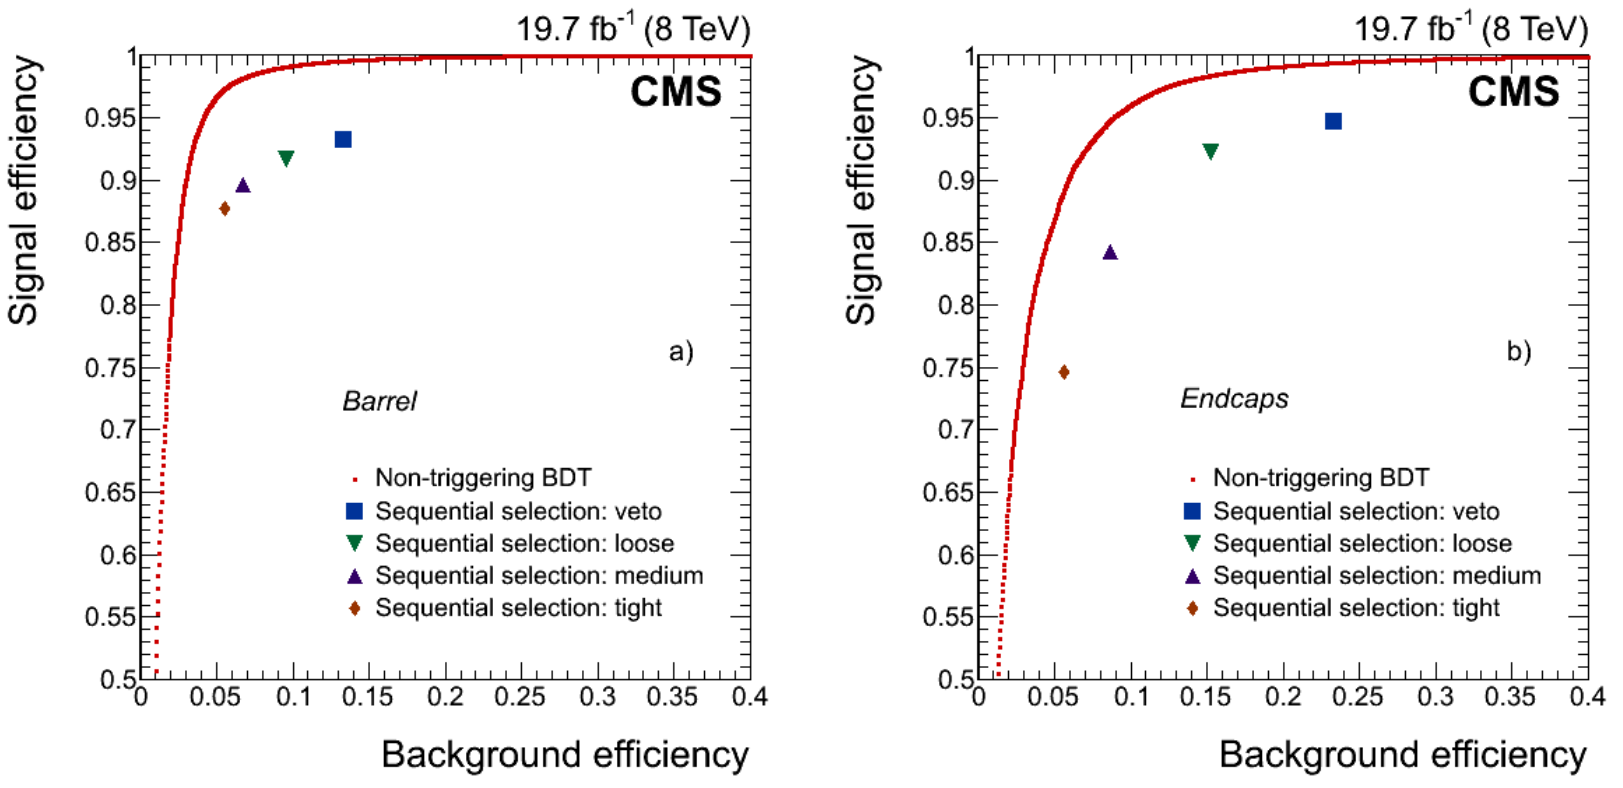
\includegraphics[width=0.95\textwidth]{plots_and_figures/chapter4/elec_eff.png}
\caption{Performance of the BDT-based electron identification algorithm (red dots) compared with results from several working points of cut-based selection for electron candidates in the ECAL barrel (left), and endcaps (right)~\cite{e_recon}.}
 \label{fig:elec_eff}
\end{figure*}


\subsection{Hadronic tau leptons}
\label{tau_recon}
Tau leptons decay hadronically in several ways or decay modes. The primary decay modes consist of: one charged hadron and up to two neutral pions, or three charged hadrons. The algorithm that is used to reconstruct hadronically decaying tau leptons in CMS is called the hadrons-plus-strips (HPS) algorithm~\cite{Khachatryan:2015dfa,Sirunyan:tau16}. This algorithm proceeds in two steps. In the first step, the topology of the candidate is checked to match the topology of one of the decay modes. The second step consists of a MVA-based discriminator (built using variables such as lifetime information, decay mode etc.), that is used to reject electrons, muons, quarks or gluon jets wrongly identified as hadronic taus. The reconstruction efficiency is also improved, in the case of converted photons from a neutral-pion decay, by considering PF photons and electrons from a strip along the $\phi$ direction. The final states in the analyses presented here do not contain hadronically decaying taus. Hence, all events which contain hadronically decaying taus are rejected.


\subsection{Jet reconstruction}
\label{jet_recon}
Jets are clusters of particles that are experimental signatures of quark and gluons which hadronize (due to color confinement) producing a narrow spray or ``jet'' of particles~\cite{jet_recon}. Jets are reconstructed in CMS by clustering PF objects. In order to group together objects into a jet, CMS uses the anti-$k_{T}$ clustering algorithm. This belongs to a broader class of clustering algorithms called sequential clustering algorithms which cluster objects into jet in a sequential order following a predefined set of rules. The general form of a sequential clustering algorithm is based on the quantities  $d_{ij}$, which represents the distance between two entities, and $d_{iB}$ which represents the distance of the i-th entity from the beam axis. These distances are defined as:
\begin{equation}
  d_{ij}=min(k_{ti}^{2p},k_{tj}^{2p})\frac{\Delta_{ij}^{2}}{R^2}
\end{equation}
\begin{equation}
  d_{iB}=k_{ti}^{2p}
\end{equation}
where $\Delta_{ij}^{2}=(\eta_i-\eta_j)^2+(\phi_i-\phi_j)^2$, $k_{ti}$ is the transverse momentum of the i-th entity and R is the radius parameter which is set as 0.4. The parameter p governs the relative power of energy versus geometrical scales and the particular value of $p=-1$ defines the anti-$k_{T}$ clustering algorithm. The algorithm first computes distance $d_{ij}$ between all entity pairs present at that stage. If the minimum of those distances (say between entity i and j) is smaller than the minimum distance $d_{iB}$ of any entity from the beam axis, those entities i and j are combined into a single entity. Otherwise, the entity closest to the beam axis is considered a jet and removed from the list of entities to be further clustered. This continues until all entities are clustered. The anti-$k_{T}$ is dominated by high $\pt$ particles which it clusters first, subsequently including softer and softer constituents. Soft particles tend to cluster with hard particles before they tend to cluster among themselves. A hard particle that has no hard neighbors within a distance 2R accumulates all the soft particles within a circle of radius R. It tries to produce jets with fairly conical shapes that are centered around the hardest particles of the event, and with boundaries that resilient to the effect of soft radiation.

Jets being complex objects suffer from several effects that cause their energy, reconstructed as described above, to differ from their true values. Multiplicative correction factors are applied to calibrate their $\pt$ and to ensure a uniform response in $\eta$~\cite{jet_recon1,jet_recon2}. A total of four multiplicative corrections are applied. Firstly, the energy coming from pileup that has been clustered into the jet needs to be corrected for. A correction is applied based on the \textit{hybrid jet area} method which is a combination of two methods viz., the average offset method and the jet area method. The average offset method uses zero bias events to measure the average amount of energy added to the event due to pileup. The assumption is that averaging over zero bias events makes this measurement insensitive to high $\pt$ objects and primarily represents soft pileup contributions. The average offset is measured in bins of $\eta$ and number of pileup vertices ($N_{PV}$) averaged over $\phi$. The correction is then given by $1-\frac{<Offset(N_{PV},\eta)>}{p_{T}^{RAW}}$, where $p_{T}^{RAW}$  is the uncorrected jet $\pt$. The drawback of this method is that it assumes that every jet contains the same amount of pileup contribution. The jet area method, on the other hand , calculates corrections on a jet-by-jet basis. It calculates an energy density  per event  by clustering jets using the $k_{T}$ algorithm (this has a value of parameter p=1 and favors clustering soft jets as opposed to hard ones) and dividing the $\pt$ by jet area, which is defined as the region in $\eta-\phi$ occupied by soft particles clustered in the jet. The median of this distribution ($\rho$) for an event is expected to be insensitive to hard particles and thus $\rho A_{j}$ is a good approximation of pileup contribution to the i-th jet. The drawback of this second approach, however is that it doesn't take into account the fact that the detector response is $\eta$ dependent. The \textit{hybrid jet area} method combines these two methods to calculate a jet-by-jet correction depending on $\eta$ and $N_{PV}$. Secondly, a MC calibration factor, which corrects the energy of reconstructed jets to match the generated MC particle jet energy on average, is applied. This factor is based on simulated events. Finally, two other factors are used that each calibrate the energy response of reconstructed jets to be uniform with respect to $\eta$ and $\pt$. These are also measured using simulated events. A QCD dijet sample is used to uniformize the dependence in $\eta$. Conservation of momentum in the transverse plane tells us that the sum of momentum in the transverse plane should be zero. Using jets that are approximately back-to-back in the azimuthal direction but at different $\eta$ regions of the detector, the difference in response between these two $\eta$ regions can be ascertained and corrected/uniformized. Using the same method of measuring residual response in the transverse direction in $\gamma + jets$ or $Z +jets$  events, the absolute jet energy scale as a function of $\pt$ can be made uniform.


\subsection{Missing transverse energy: \ptvecmiss} 
\label{mt_met_recon}
The CMS detector is unable to detect neutrinos (and other hypothetical particles) that are weakly interacting. However, the momentum balance (or imbalance) in the plane transverse to beam direction can be used to infer their presence. This ``missing'' transverse momentum vector is referred to as the \ptvecmiss and its magnitude is referred to as \ptmiss. It is defined as the negative vector sum of the $\pt$ of entire list of objects reconstructed in the event by the above reconstruction algorithms and refined by particle-flow (PF objects):
\begin{equation}
  \ptvecmiss=-\Sigma\ptvec
\end{equation}
The \ptvecmiss plays an important role in this analysis as it helps gauge the momentum of the neutrinos from the decaying tau lepton. The \ptvecmiss reconstruction is directly dependent on the reconstruction of all the other objects in the event, from jets to muons to electrons. Consequently, it is sensitive to all the effects that influence the precise reconstruction and calibration of these objects. The largest effects come from biases in jet reconstruction and pileup (which are interconnected). Jet energy corrections described in previous section and pileup mitigation techniques discussed earlier can help significantly reduce the bias in \ptvecmiss reconstruction~\cite{Sirunyan:2019kia}. 


\subsection{Relative isolation}
\label{isolation}
The isolation of an object is the measure of the absence of other objects in its vicinity. In other words, it is the measure of how ``isolated'' an object is. It is calculated by summing up the $\pt$ of all objects in a cone with predefined radius $\Delta R=0.4$ around the lepton. The relative isolation which is obtained by dividing the isolation by the $\pt$ of the lepton is then given by:

\begin{equation}
I_\text{rel}^{\ell} = \left( \sum  \pt^\text{charged} + \text{max}\left[ 0, \sum \pt^\text{neutral}
                                 +  \sum \pt^{\gamma} - \pt^\text{PU}\left(\ell\right)  \right] \right) /  \pt^{\ell},
\end{equation}

where $\pt^\text{charged}$, $\pt^\text{neutral}$, and $\pt^{\gamma}$  indicate the $\pt$ of a charged particle, a neutral particle, and a photon within the cone, respectively. The contribution to isolation sum from charged particles in the cone coming from pileup is excluded by requiring the track origins be consistent with the primary vertex associated with the hard interaction. However, the same procedure cannot be adopted for neutral particles in the cone coming from pileup. This contribution, $\pt^\text{PU}\left(\ell\right)$, is estimated using a jet area method for electrons~\cite{isolation_1,isolation_2}, and simply as half of the scalar $\pt$ sum of charged particles from pileup inside the cone for muons. The definition ensures that the total contribution to the isolation cone sum for neutral particles is always greater than or equal to 0. 

The relative isolation is an useful variable in this analysis as prompt objects are usually isolated. More importantly, for an analyses with electrons and muons in the final state such as this, a tightened isolation requirement helps to reject those events where a jet is misidentified as either one of these leptons. Strict isolation requirements are thus used in the event selection in this analysis as described in sections ~\ref{h125_presel_cat} and ~\ref{H_presel_cat}.    




\subsection{Collinear mass: \mcol and transverse mass: $M_{T}$}
\label{col_mass}
An important variable of interest in this analysis is the collinear mass, $\mcol$. As mentioned in later chapters, $\mcol$ is used as the signal variable in the $\Hmue$ analysis and in the $\mcol$ fit method of the $\hmue$ analysis. The visible mass of the muon-electron system, $\mvis$ is not a very good estimator of the Higgs boson mass. This is because the neutrinos from the tau decay do not interact with the detector and the energy they carry is ``lost''. $\mcol$ provides a better estimate of the Higgs mass by approximating the neutrino momenta using the collinear approximation~\cite{Ellis:1987xu}. The primary idea is the following. The mass of the Higgs being much larger than that of the tau lepton causes the tau lepton to become highly boosted. Consequently, the decay products of the tau lepton, i.e. the electron, the tau neutrino and the electron neutrino, are produced in a highly collimated region around the direction of the tau lepton momentum. The momenta of the neutrinos ($\pt^{\nu,\,\text{est}}$) can thus be approximated from the projection of \ptvecmiss in the direction of momenta of the visible tau decay product (electron), i.e. $\vec{\pt^{\Pe}}$. The visible fraction of the tau lepton momentum is then given as $x_{\Pgt}^\text{vis}={\pt^{\vec{\Pgt}^{\text{vis}}}}/{(\pt^{\vec{\Pgt}^\text{vis}}+\pt^{\nu,\,\text{est}})}$. Finally, $\mcol$ is given as $M_{\text{col}}= M_{\text{vis}} / \sqrt{\smash[b]{x_{\Pgt}^\text{vis}}}$. A very simple illustration in Figure~\ref{fig:mcol_v_mvis} shows the superimposition  the $\mcol$ and $\mvis$ spectrums for a 300 GeV Higgs boson. Evidently, $\mcol$ is a better estimator of the mass and also has a sharper peak.

\begin{figure*}[!htpb]\centering
 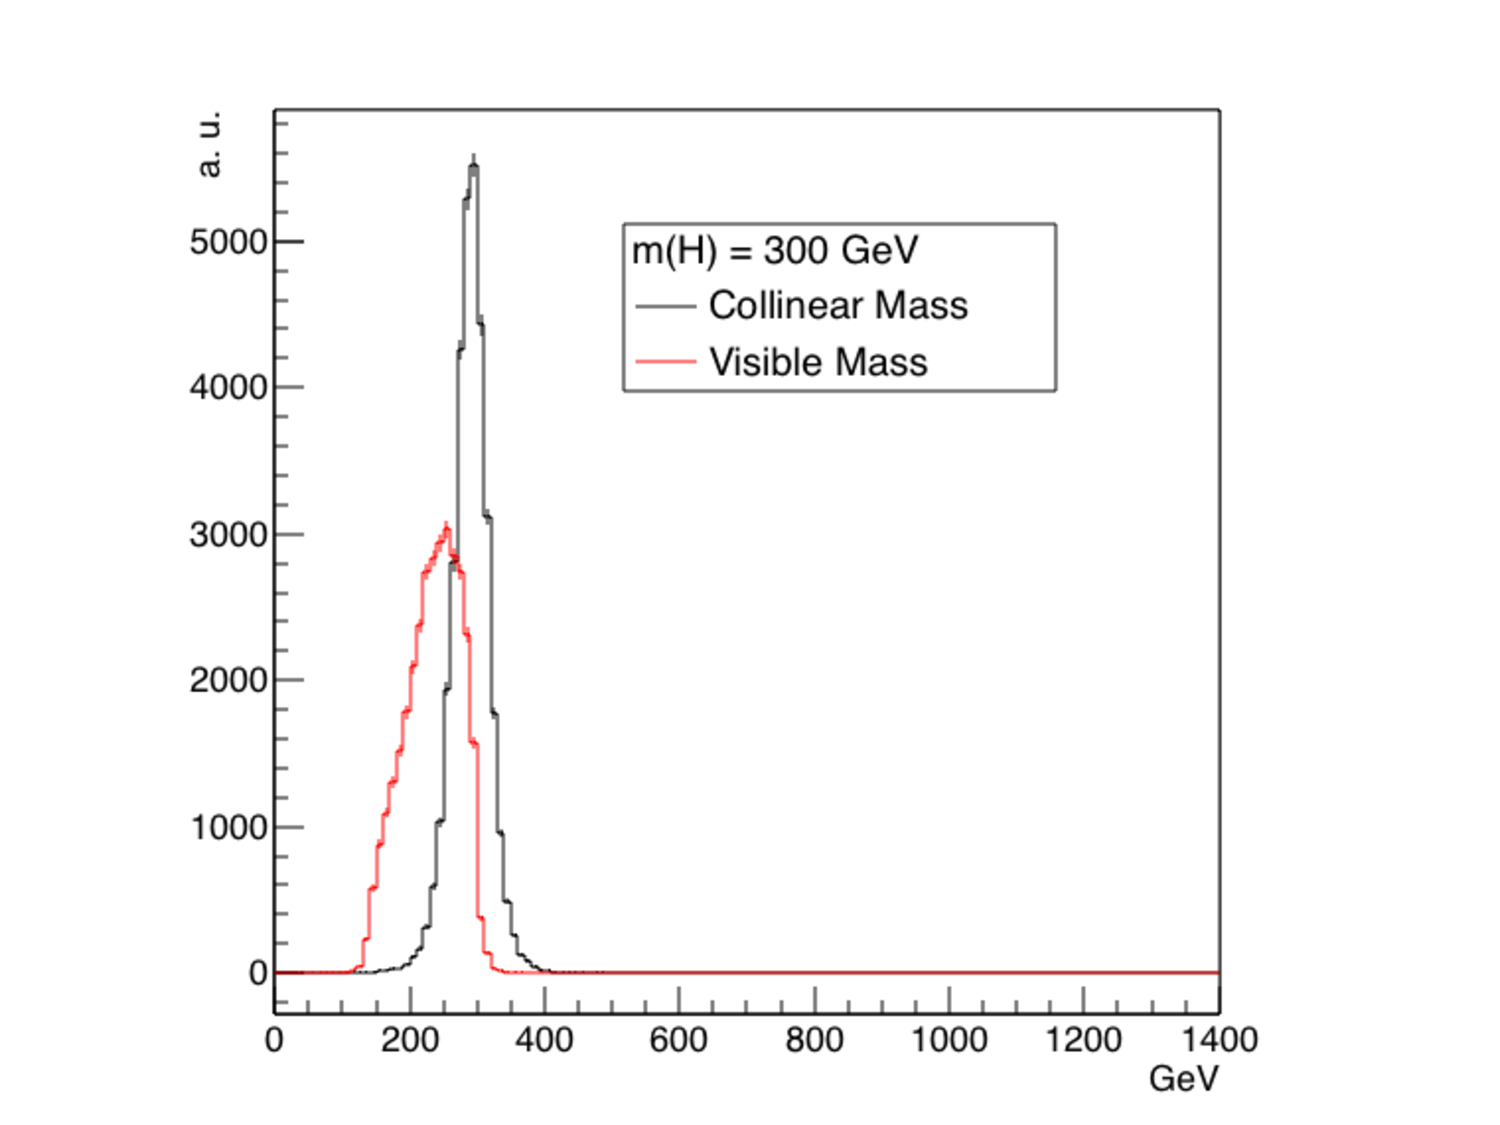
\includegraphics[width=0.9\textwidth]{plots_and_figures/chapter4/mcol_v_mvis.pdf}
\caption{\mcol and \mvis distributions for Higgs mass of 300 GeV.}
 \label{fig:mcol_v_mvis}
\end{figure*}


Another variable that is used in this analyses and is useful to discriminate signal from background (see chapter~\ref{evt_sel}) is the transverse mass, $\mt(\ell)$ ($\ell = \Pgm, \Pe$). It is defined as follows: $ {\mt}(\ell)=\sqrt{\smash[b]{2|\ptvec^{\ell}||\ptvecmiss|(1-\cos{\Delta \phi_{\ell - \ptmiss}})}} $, where $\Delta \phi_{\ell - \ptmiss}$ is the angle between the lepton transverse momentum and \ptvecmiss.


% % uncomment the following lines,
% if using chapter-wise bibliography
%
% \bibliographystyle{ndnatbib}
% \bibliography{example}

% % uncomment the following lines,
% if using chapter-wise bibliography
%
% \bibliographystyle{ndnatbib}
% \bibliography{example}
